%
% Niniejszy plik stanowi przykład formatowania pracy magisterskiej na
% Wydziale MIM UW.  Szkielet użytych poleceń można wykorzystywać do
% woli, np. formatujac wlasna prace.
%
% Zawartosc merytoryczna stanowi oryginalnosiagniecie
% naukowosciowe Marcina Wolinskiego.  Wszelkie prawa zastrzeżone.
%
% Copyright (c) 2001 by Marcin Woliński <M.Wolinski@gust.org.pl>
% Poprawki spowodowane zmianami przepisów - Marcin Szczuka, 1.10.2004
% Poprawki spowodowane zmianami przepisow i ujednolicenie 
% - Seweryn Karłowicz, 05.05.2006
% Dodanie wielu autorów i tłumaczenia na angielski - Kuba Pochrybniak, 29.11.2016

% dodaj opcję [licencjacka] dla pracy licencjackiej
% dodaj opcję [en] dla wersji angielskiej (mogą być obie: [licencjacka,en])
\documentclass[en]{pracamgr}

% Dane magistranta:
\autor{Katarzyna Kowalska}{371053}

% Dane magistrantów:
%\autor{Autor Zerowy}{342007}
%\autori{Autor Pierwszy}{342013}
%\autorii{Drugi Autor-Z-Rzędu}{231023}
%\autoriii{Trzeci z Autorów}{777321}
%\autoriv{Autor nr Cztery}{432145}
%\autorv{Autor nr Pięć}{342011}

\title{Approximation and Parametrized Algorithms for Geometric Set Cover}
\titlepl{Algorytmy parametryzowania i
trudność aproksymacji problemu pokrywania zbiorów na płaszczyźnie}

%\tytulang{An implementation of a difference blabalizer based on the theory of $\sigma$ -- $\rho$ phetors}

%kierunek: 
% - matematyka, informacyka, ...
% - Mathematics, Computer Science, ...
\kierunek{Computer Science}

% informatyka - nie okreslamy zakresu (opcja zakomentowana)
% matematyka - zakres moze pozostac nieokreslony,
% a jesli ma byc okreslony dla pracy mgr,
% to przyjmuje jedna z wartosci:
% {metod matematycznych w finansach}
% {metod matematycznych w ubezpieczeniach}
% {matematyki stosowanej}
% {nauczania matematyki}
% Dla pracy licencjackiej mamy natomiast
% mozliwosc wpisania takiej wartosci zakresu:
% {Jednoczesnych Studiow Ekonomiczno--Matematycznych}

% \zakres{Tu wpisac, jesli trzeba, jedna z opcji podanych wyzej}

% Praca wykonana pod kierunkiem:
% (podać tytuł/stopień imię i nazwisko opiekuna
% Instytut
% ew. Wydział ew. Uczelnia (jeżeli nie MIM UW))
\opiekun{dr Michał Pilipczuk\\
  Instytut Informatyki\\
  }

% miesiąc i~rok:
\date{June 2020}

%Podać dziedzinę wg klasyfikacji Socrates-Erasmus:
\dziedzina{ 
%11.0 Matematyka, Informatyka:\\ 
%11.1 Matematyka\\ 
%11.2 Statystyka\\ 
11.3 Informatyka\\ 
%11.4 Sztuczna inteligencja\\ 
%11.5 Nauki aktuarialne\\
%11.9 Inne nauki matematyczne i informatyczne
}

%Klasyfikacja tematyczna wedlug AMS (matematyka) lub ACM (informatyka)
\klasyfikacja{D. Software\\
  D.127. Blabalgorithms\\
  D.127.6. Numerical blabalysis}

% Słowa kluczowe:
\keywords{blabaliza różnicowa, fetory $\sigma$-$\rho$, fooizm,
  blarbarucja, blaba, fetoryka, baleronik}

% Tu jest dobre miejsce na Twoje własne makra i~środowiska:

\newcommand{\points}{\mathcal{C}}
\newcommand{\sets}{\mathcal{P}}
\newcommand{\sol}{\mathcal{R}}

\usepackage{amsfonts}
\usepackage{amsmath}
\usepackage{graphicx}
\newtheorem{defi}{Definition}[section]
\newtheorem{tw}{Theorem}[section]
\newtheorem{lemma}{Lemma}[section]

% koniec definicji

\begin{document}
\maketitle

%tu idzie streszczenie na strone poczatkowa
\begin{abstract}
  W~pracy przedstawiono prototypową implementację blabalizatora
  różnicowego bazującą na teorii fetorów $\sigma$-$\rho$ profesora
  Fifaka.  Wykorzystanie teorii Fifaka daje wreszcie możliwość
  efektywnego wykonania blabalizy numerycznej.  Fakt ten stanowi
  przełom technologiczny, którego konsekwencje trudno z~góry
  przewidzieć.
\end{abstract}

\tableofcontents
%\listoffigures
%\listoftables

\chapter{Introduction}
This is some very boring and really nothing on the topic introduction.
\chapter{Definitions}
Some definitions what geometric set cover is.
$\sets$ -- set of objects, $\points$ -- set of points.
Choose $\sol \subset \sets$ such that
every point in $\points$ is inside some element from $\sol$
and $|\sol|$ is minimal.

In parametrized setting we only look among $|\sol| \le k$.
In weighted settings there is some $f : \sets -> \mathbb{R}$
and we minimize $\sum_{R \in \sol} f(R)$.
 
\chapter{Geometric Set Cover with segments}

\section{FPT for segments}
\subsection{Segments parallel to one of the axis}
You can find this in Platypus book.

We'll show $\mathcal{O}(2^k)$ branching algorithm.
Let's take point $K$ that hasn't been covered yet with
the smallest coordinate in lexicograpical order.
We need to cover $K$ with some of the remaining segments.

We choose one of the 2 directions on which we will cover this point.
In this direction we take greedly the segment that will cover
the most points (there are points in $\points$ only on
one side of $K$ in this direction, so all
segments covering $K$ in this direction create monotone sequence
of sets -- zbiory zstępujące).

\subsection{Segments in $d$ directions}
The same algorithm as before but in complexity $\mathcal{O}(d^k)$.

\subsection{Segments in arbitrary direction}
If there exist two segments $a$ and $b$ in $\sets$,
such that any point covered by $a$ is also covered by $b$,
then without loss of generality we can remove segment $a$ from $\sets$.
We repeat this process until no such $(a, b)$ pair exists.


Let us first assume that we reduced our instance to a kernel,
where \textit{any line} contains no more than $k$ points.

Since any segment covers a set of colinear points,
for such a kernel $k$ segments can cover only at most $k^2$ points.
Therefore, for the answer to be positive,
the number of points has to be at most $k^2$.
The number of segments is now bounded by $k^4$,
since if we consider two \textit{extreme} points
covered by a given segment,
then these pairs must be distinct,
otherwise two segments would contain the same set of points.
Since both the number of points and the number of segments
is bounded by a function of $k$,
this instance can be easily solved in time $O(f(k))$.

In remains to show how to construct the kernel.

%As long as there is a line with more than $k$ points, do branching.
%Let's name points on this line $x_1, x_2, \ldots x_t$
%in order they appear on the line.

%So we choose on which point the chosen segment on this line
%will start. Of course we have to take at least one segment
%covering at least one point among first $k+1$ points,
%because covering all of them with only segments
%on different lines we would use
%exactly $k+1$ segments (any of them can't contain more than
%one point from this line).


Assume there exists a line $l$ containing points $x_1$, \ldots $x_t$,
where $t \geq k + 1$.
Note that a segment that does not lie on $l$ can cover only at most one
of the points $x_i$.
Therefore, out of points $x_1$, ..., $x_{k+1}$,
at least one has to be covered by a segment that lies on $l$,
let us fix $x_i$ to be the first such point.
Then, we can greedily choose a segment that lies on $l$,
covers $x_i$,
and also covers the largest number of points $x_j$ for $j > i$.

Since we have at most $k + 1$ choices to branch over
and each choice adds a segment to the constructed solution,
we obtain an algorithm with complexity $O(k^k)$.

\section{APX-completeness for segments pararell to axis}
\label{section:segment_apx}
It works even with extensions for unit weights.

We will show reduction from MAX-(3,3)-SAT
to Geometric Set Cover with segments pararell to axis.

\subsection{Definition of  MAX-(3,3)-SAT problem}
Here we define MAXSAT problem.

\subsection{Reduction construction}

Let's take some instance of  MAX-(3,3)-SAT with
variables $x_1, x_2 \ldots x_n$
and clauses $C_1, C_2 \dots C_n$.

We will create gadgets for choosing the value
of variables (\textit{true} or \textit{false}) and checking
if the clauses are met (any of the variables were chosen).

\begin{figure}[h]
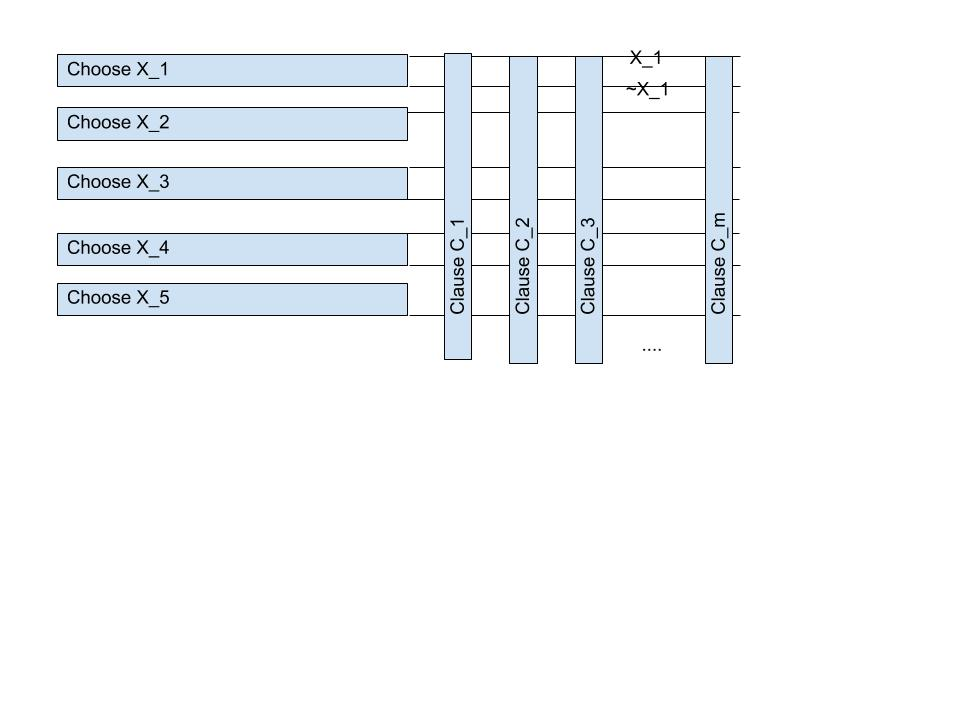
\includegraphics[width=0.7\textwidth]{segment_apx_sketch.jpg}
\caption{General scheme of reduction.}
\label{fig:segment_apx}
\end{figure}

\subsubsection{Choose $x_i$ gadget}
\begin{figure}[h]
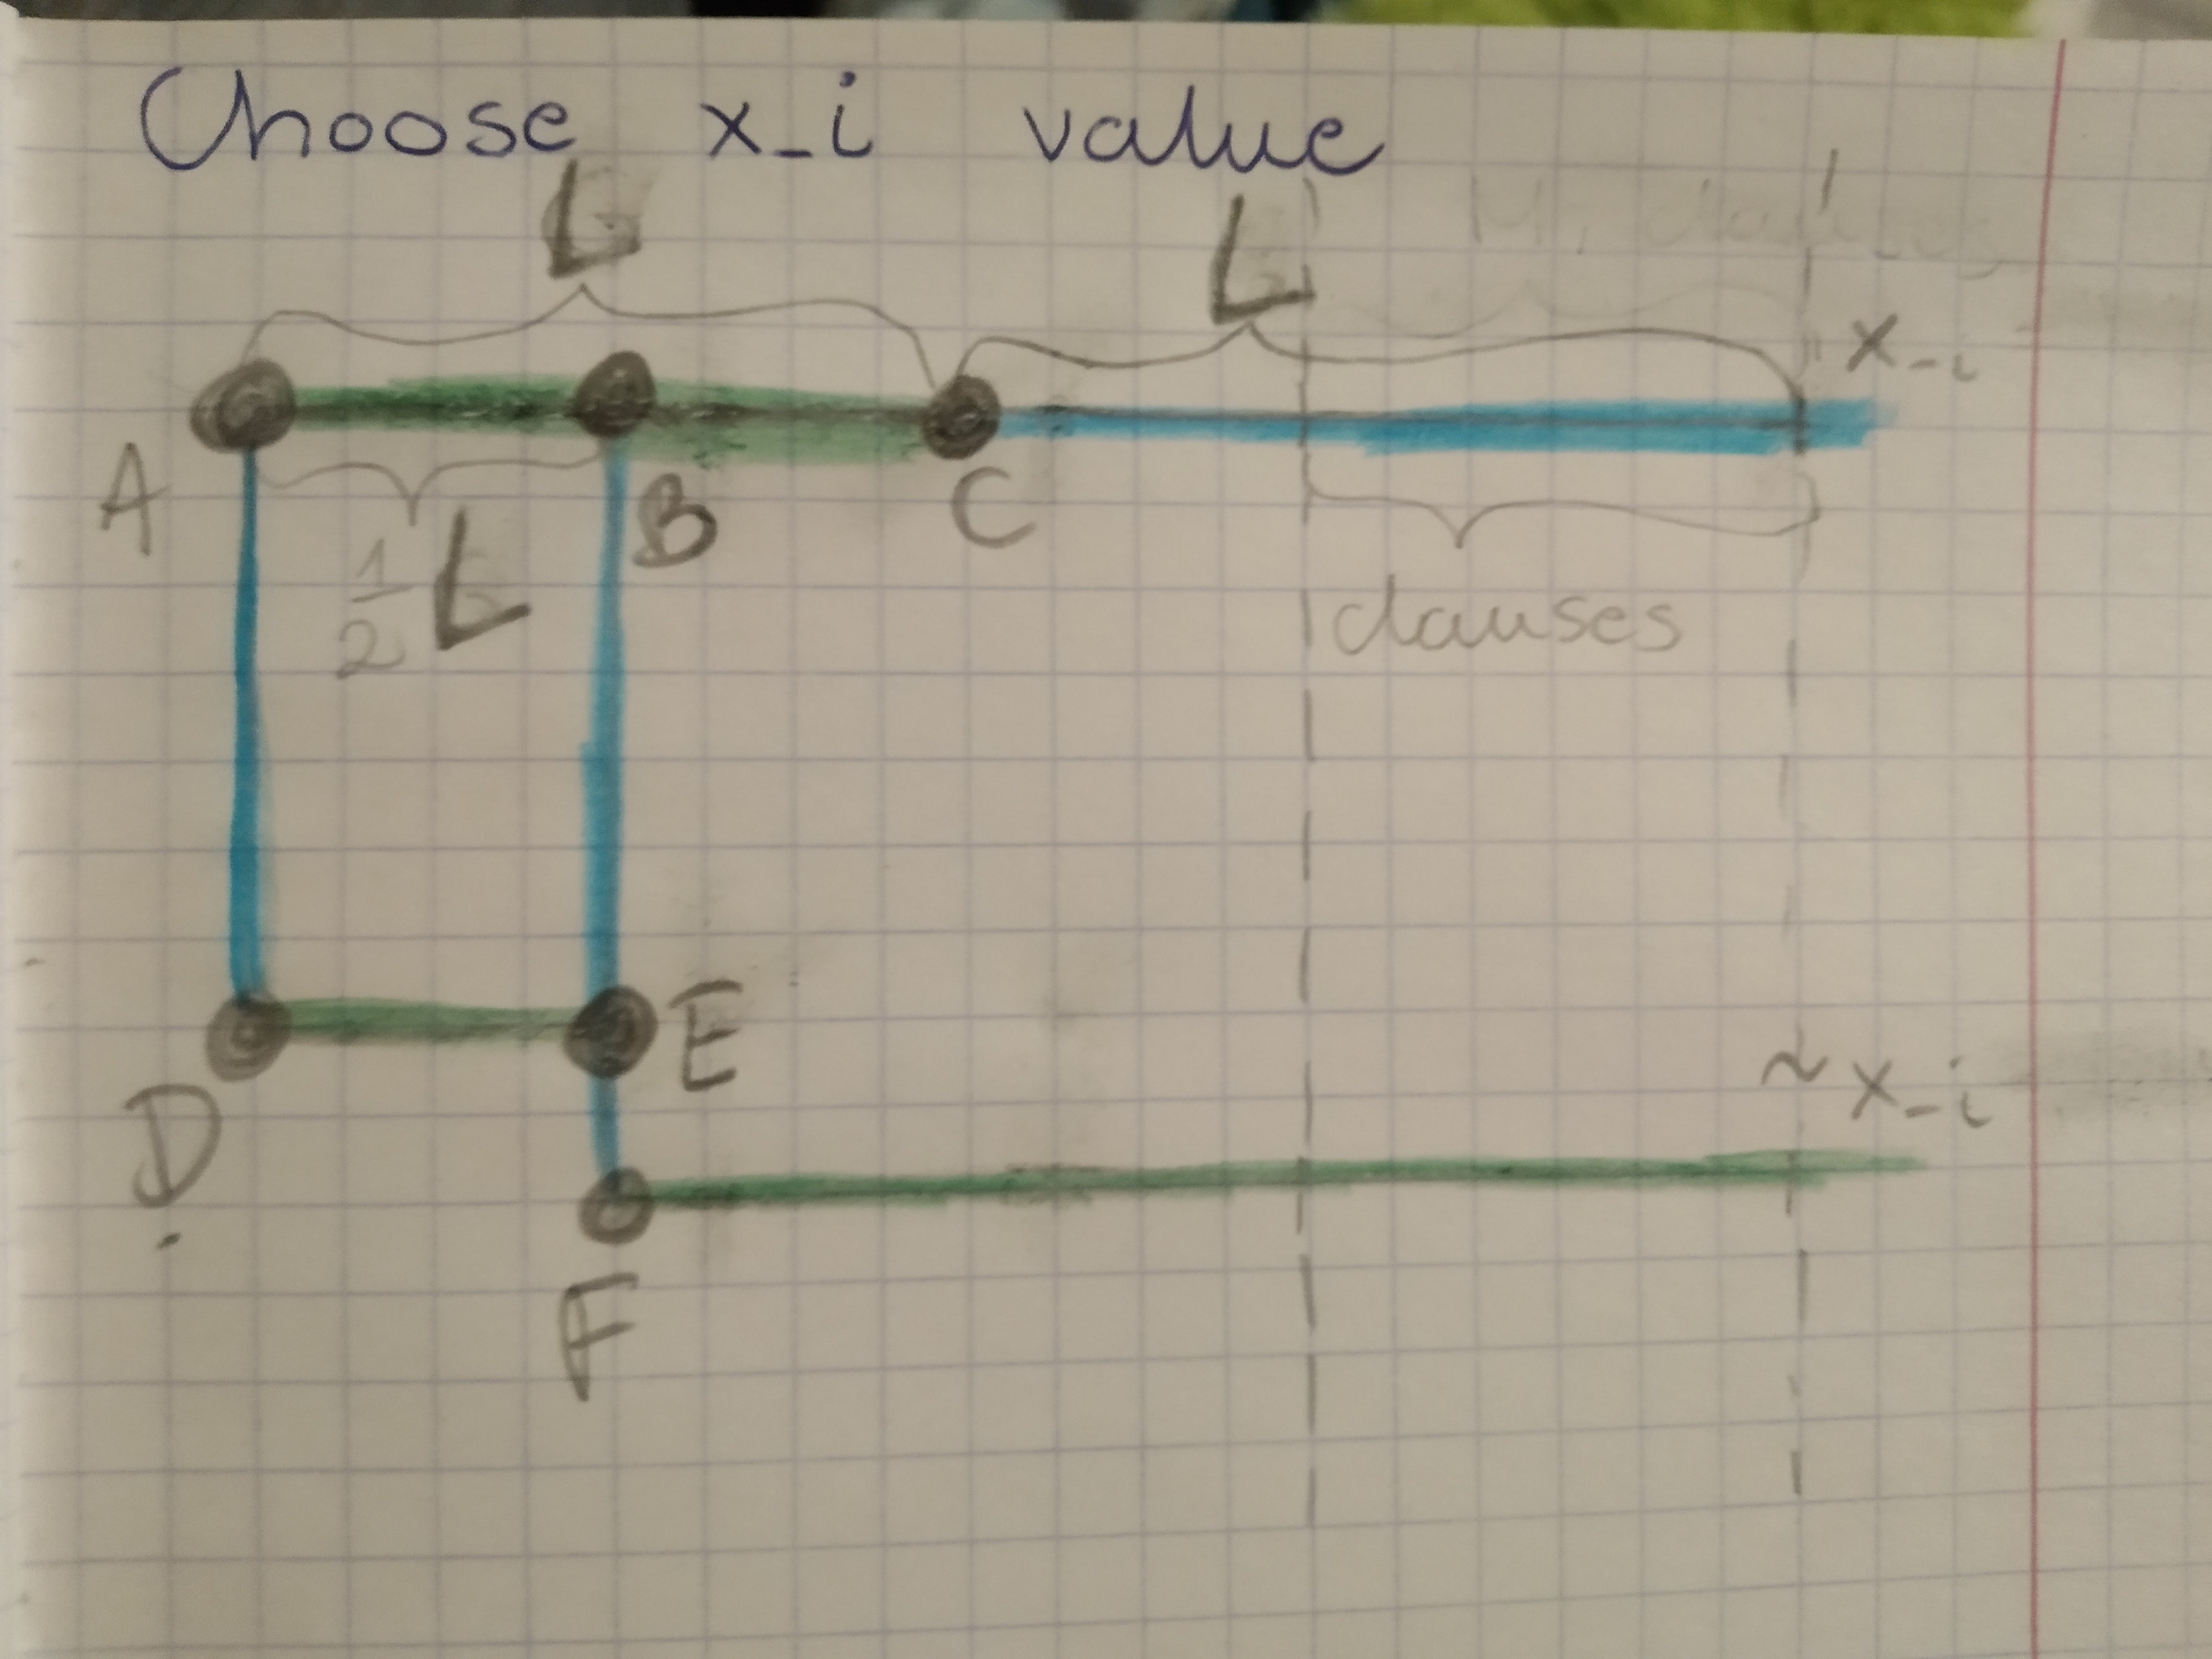
\includegraphics[width=0.6\textwidth]{choose_x_gadget.jpg}
\caption{Scheme of choose $x_i$ gadget.}
\label{fig:choose_x_gadget}
\end{figure}
In Figure~\ref{fig:choose_x_gadget},
we show a gadget that simulates a single variable $x_i$.
It consists of six points A, B, C, D, E, F, and several segments.
Selecting the segment marked with $x_i$
to the solution will correspond to setting $x_i$ to \textit{true},
while selecting the segment marked with $\neg x_i$
to setting $x_i$ to \textit{false}.
In the following lemmas,
we show that this construction indeed models a binary variable.

First, note that in the gadget
there are exactly two sets of three segments
that cover all points $A, B, C, D, E, F$.
These two sets of segments are marked in
Figure~\ref{fig:choose_x_gadget} in blue and green, respectively.

\begin{lemma}
Points $A, B, C, D, E, F$ cannot be covered using less than
3 segments (even with $1/2$-extensions).
\end{lemma}
\paragraph{Proof.}
We need to take at least one segment on line $ABC$,
because it's the only way to cover $C$.
All other points ($D, E, F$) are not colinear,
so we need at least 2 other segments to cover them.

\begin{lemma}
If we choose both segments $x_i$ and $\neg x_i$, we need to use at
least 4 segments to cover all points $A, B, C, D, E, F$
(even with $1/2$-extensions).
\end{lemma}

\paragraph{Proof.}
Choosing both segments $x_i$ and $\neg x_i$
we only cover points $C$
(becuase $B$ is too far away to be covered with $1/2$-extension)
and $F$.

The remaining points ($A, B, D, E$) are not colinear,
so we need at least two more segments to cover them.

\paragraph{Robustness to $1/2$-extension.}
Take a look at Figure~\ref{fig:segment_apx}.
The points will be included in choose gadgets (horizontal boxes)
and clause gadgets (vertical boxes).

Since segment $AC$ is very long
and colinear with $x_i$, after $1/2$-extension
it will cover a significant part of segment $x_i$,
even though $x_i$ will not be chosen.

If we put all the clause gadgets in the area
marked with \textbf{clauses} at gadget scheme in Figure~\ref{fig:choose_x_gadget},
it is enough to prove that $AC$ will not cover any points
in the \textbf{clauses} area even with $1/2$-extensions.

\begin{lemma}
No points in \textbf{clauses} area can be covered
by $AC$ with $1/2$-extension.
\end{lemma}

\paragraph{Proof.}
Bear in mind that length of $AC$ is equal to length of $x_i$.
Area \textbf{clauses} takes a second half
of the segment $x_i$ and $AC$ after extension will cover the first
half of segment $x_i$.

\subsubsection{Clause gadget}
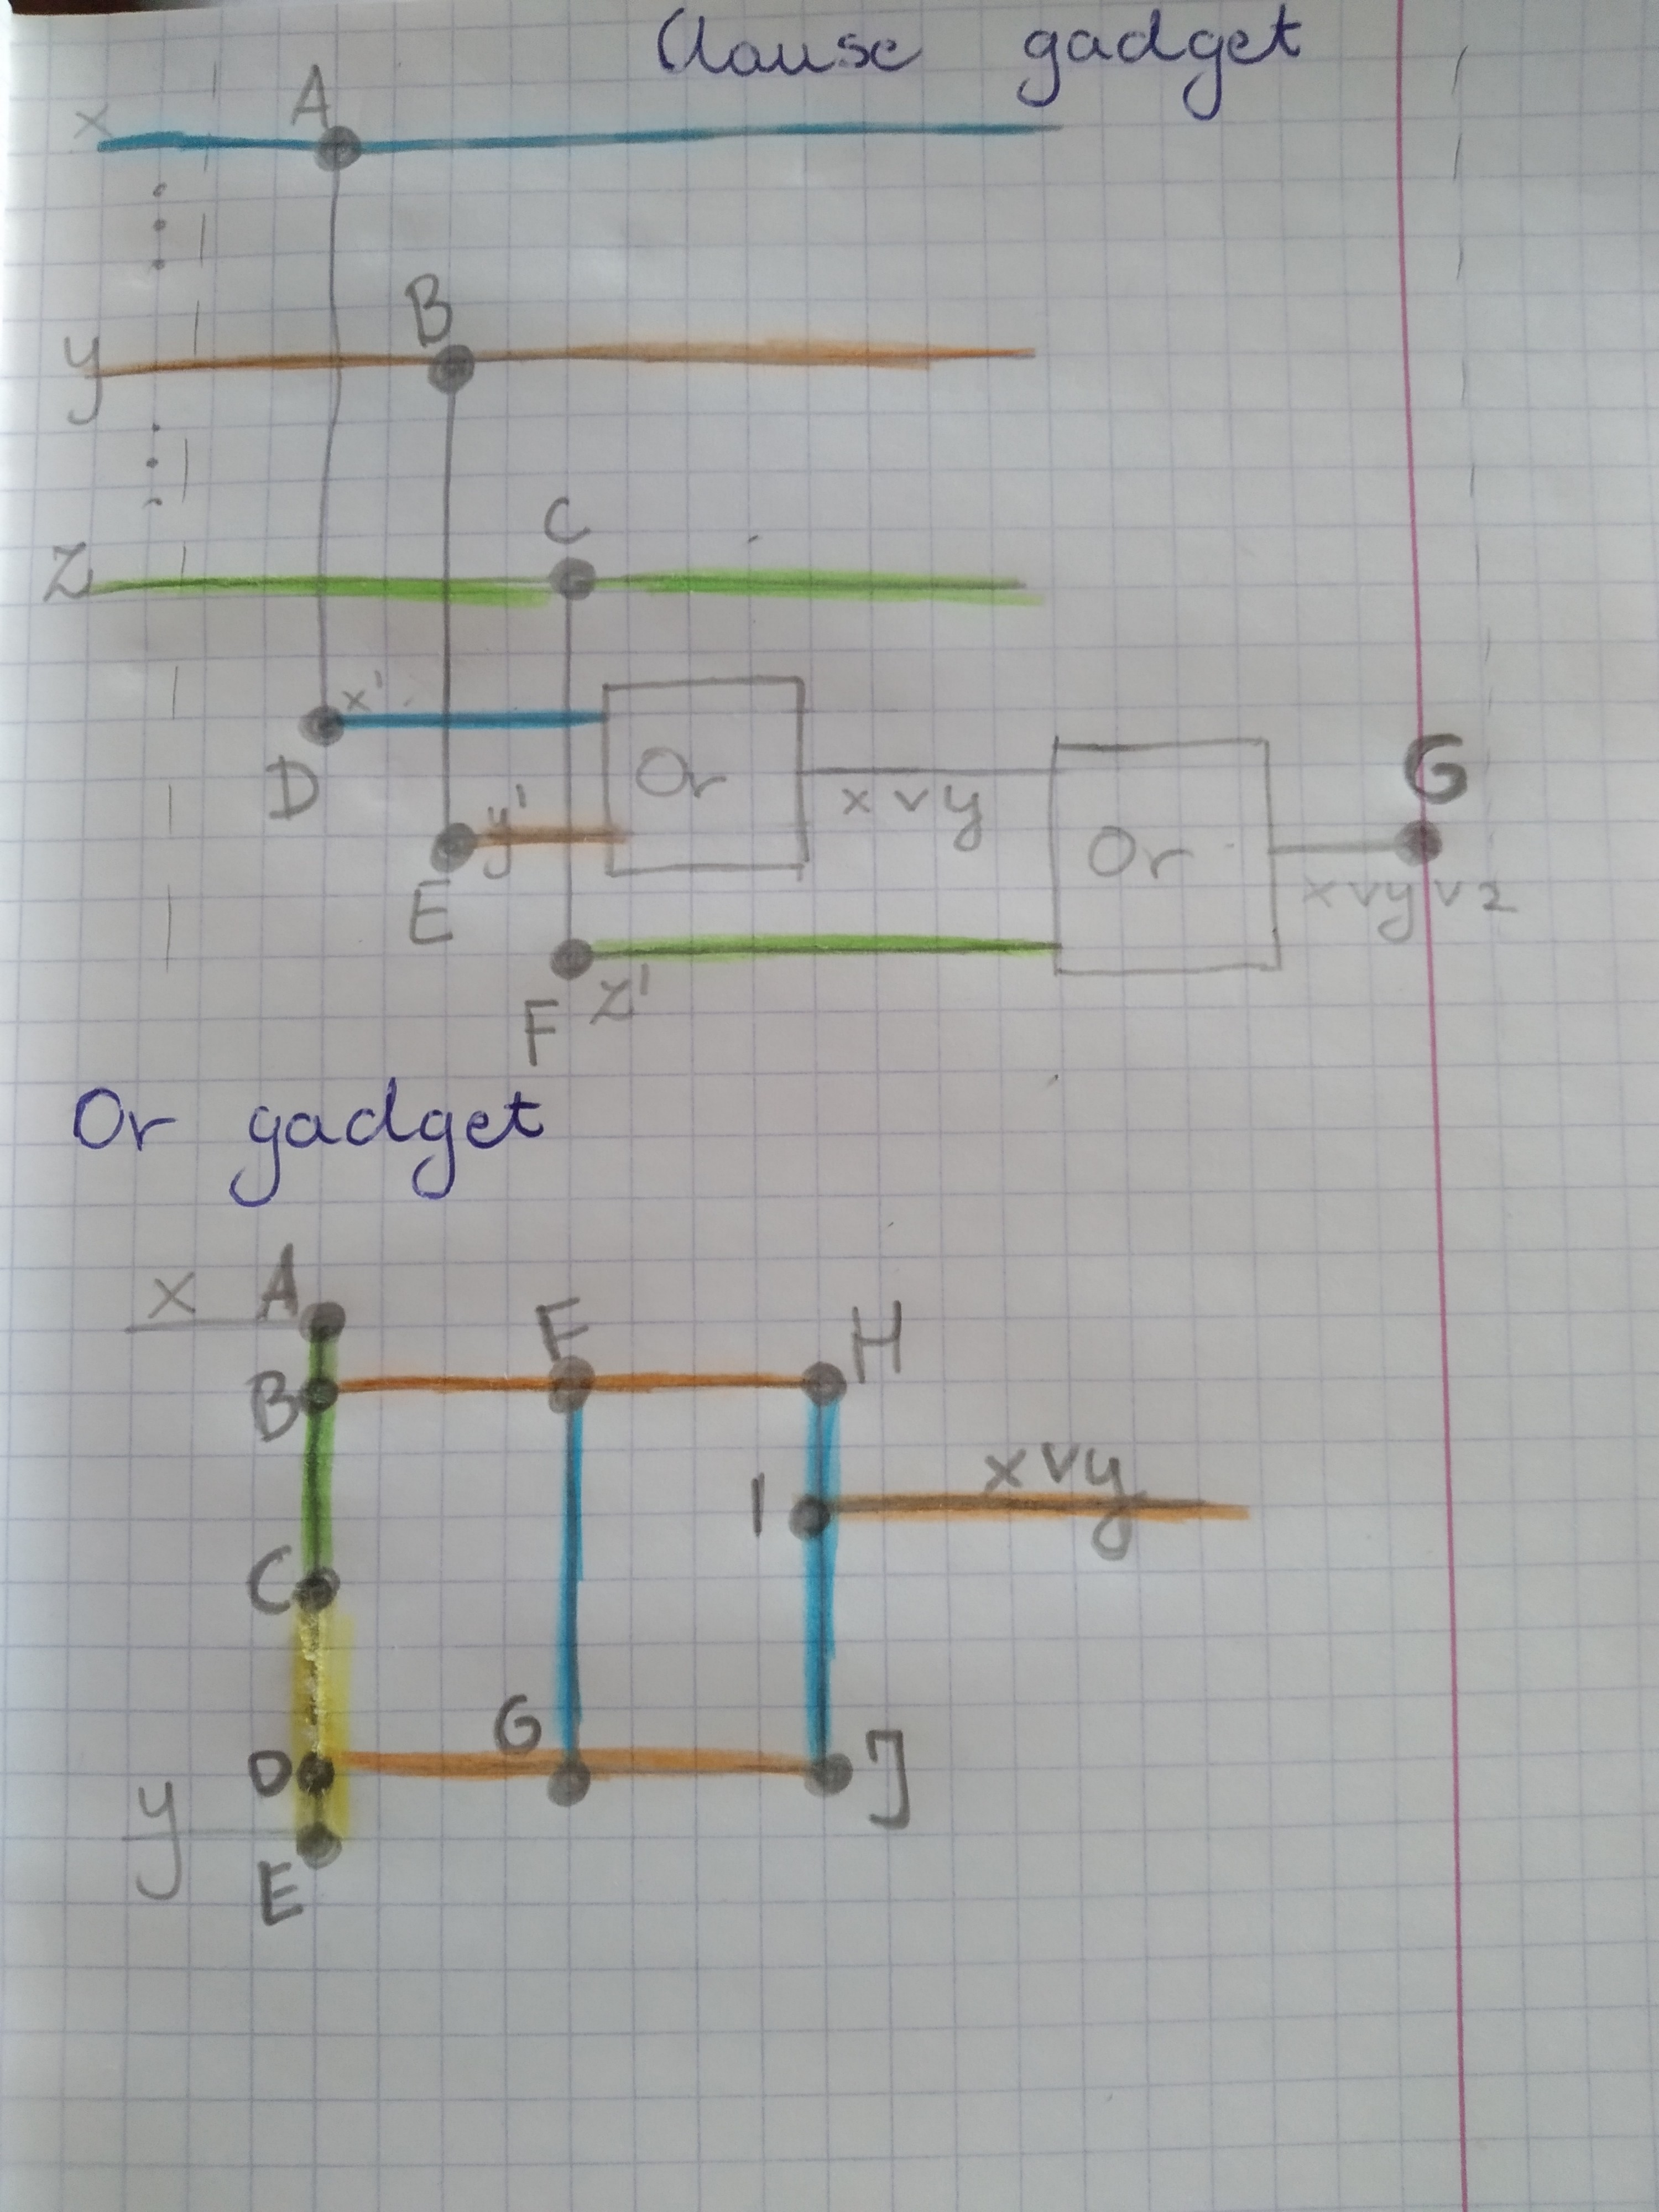
\includegraphics[width=0.6\textwidth]{clause_gadget.jpg}

\begin{lemma}
In order to cover $D$ ($E, F$) point at least one
of the segments $AD$ ($BE, CF$) or $x'$ ($y', z'$).
\end{lemma}

\begin{lemma}
Points $A$ and $D$ can be covered
with one additional segment $x'$
only if $x$ is already chosen.
Otherwise they can be covered with one segment
only by using $AD$.
\end{lemma}

\begin{lemma}
Points $A, B, C, D, E, F, G$ can be covered with 
3 or 4 segments, depending if at least one of the segments
$x, y, z$ was previously chosen.
\end{lemma}

\subsubsection{Or gadget}
\begin{lemma}
Points $A, B, C, D, E, F, G, H, I, J$ can be covered using
at least 4 segments even with $1/2$-extension.
\end{lemma}

\begin{lemma}
Points $A, B, C, D, E, F, G, H, I, J$ can be covered using
4 segments and segment $x \lor y$ can be chosen
even with $1/2$-extension
only if at least one of the segments $x$ or $y$ is chosen.
\end{lemma}

\subsection{Proof that construction is sound}
\begin{lemma}
If there exists setting of values of variables that exactly $k$
clauses are satisfied, we can cover all the points
with $3n + 11m + (m-k)$ segments.
\end{lemma}

\begin{lemma}
If there exists cover with $k$ segments,
then also there exists solution for MAX-(3,3)-SAT.

TODO: Formulate this lemma better.
\end{lemma}

\section{Weights}
\subsection{FPT for segments pararell with $\delta$-extensios}
\subsection{W[1]-completeness for arbitrary segments with weights}
\subsection{What is missing}
We don't know FPT for pararell segments
and arbitrary lines with $\delta$-extensions.

\chapter{Geometric Set Cover with lines}
\section{Lines parallel to one of the axis}
When $\mathcal{R}$ consists only of lines parallel to
one of the axis, the problem can be solved in
polynomial time.

We create bipartial graph $G$ with node for every line on the input
split into sets: $H$ -- horizontal lines and $V$ -- vertical lines.
If any two lines cover the same point from $\mathcal{C}$, then
we add edge between them.

Of course there will be no edges between nodes inside $H$,
because all of them are pararell and if they share 
one point, they are the same lines. Similar argument for $V$.
So the graph is bipartial.

Now Geometric Set Cover can be solved with Vertex Cover on graph $G$.
Since Vertex Cover (even in weighted setting) 
on bipartial graphs can be solved in polynomial time.

Short note for myself just to remember how to this in polynomial time:

Non-weighted setting - Konig theorem + max matching

Weighted setting - Min cut in graph of $\neg A$ or $\neg B$
(edges directed from $V$ to $H$)

\section{FPT for arbitrary lines}
You can find this is Platypus book.
We will show FPT kernel of size at most $k^2$.

(Maybe we need to reduce lines with one point/points with one line).

For every line if there is more than $k$ points on it,
you have to take it. At the end, if there is more than $k^2$ points,
return NO.
Otherwise there is no more than $k^4$ lines.

In weighted settings among the same lines with different weights
you leave the cheapest one and use the same algorithm.

\section{APX-completeness for arbitrary lines}
We will show a reduction from Vertex Cover problem.
Let's take an instance of the Vertex Cover problem for graph $G$.
We will create a set of $|V(G)|$ pairwise non-pararell lines,
such that no three of them share a common point.

Then for every edge in $(v, w) \in E(G)$
we put a point on crossing of lines for vertices $v$ and $w$.
They are not pararell, so there exists exactly one such point
and any other line don't cover this point (any three of them don't
cross in the same point).

Solution of Geometric Set Cover for this instance would yield
a sound solution of Vertex Cover for graph $G$.
For every point (edge) we need to choose at least one of
lines (vertices) $v$ or $w$ to cover this point.

Vertex Cover for arbitrary graph is APX-complete,
so this problem in also APX-complete.

\section{2-approximation for arbitrary lines}
Vertex Cover has an easy 2-approximation algorithm,
but here very many lines can cross through
the same point, so we can do $d$-approximation,
where $d$ is the biggest number of lines crossing through the same point.
So for set where any 3 lines don't cross in the same point
it yields 2-approximation.

The problematic cases are where through all points
cross at least $k$ points and all lines have at least $k$ points on them.
It can be created by casting $k$-grid in $k$-D space on 2D space.

Greedy algorithm yields $\log |\mathcal{R}|$-approximation,
but I have example for this for bipartial graph and
reduction with taking all lines crossing through some point
(if there are no more than $k$) would solve this case.
So maybe it works.

Unfortunaly I haven't done this :(

I can link some papers telling it's hard to do.

\section{Connection with general set cover}
Problem with finite set of lines with more dimensions
is equivalent
to problem in 2D, because we can project
lines on the plane which is not perpendicular
to any plane created by pairs of
(point from $\mathcal{C}$, line from $\mathcal{P}$).

Of course every two lines have at most one common point,
so is every family of sets that have at most one point
in common equivalent to some geometric set cover with lines?

No, because of Desargues's theorem.
Have to write down exactly what configuration is banned.


\chapter{Geometric Set Cover with polygons}
\section{State of the art}

Covering points with weighted discs admits PTAS \cite{li}
and with fat polygons with $\delta$-extensions with unit weights
admits EPTAS \cite{harpeled12}.

Although with thin objects, even if we allow $\delta$-expansion,
the Set Cover with rectangles
is APX-complete (for~$\delta = 1/2$),
it follows from APX-completeness for segments with $\delta$-expansion
in Section \ref{section:segment_apx}.

Covering points with squares is W[1]-hard \cite{marx05}.
It can be proven that assuming $SETH$,
there is no $f(k)\cdot(|\points|+|\sets|)^{k-\epsilon}$ time algorithm
for any computable function $f$ and $\epsilon >0$ that decides if there
are $k$ polygons in $\sets$ that together cover $\points$,
\textit{Theorem 1.9} in \cite{voronoi}.









\chapter{Conclusions}

\begin{thebibliography}{99}
\addcontentsline{toc}{chapter}{Bibliography}

\bibitem[HarPeled12]{harpeled12} S. Har-Peled, M. Lee,,
	\textit{Weighted geometric set cover problems revisited.}
	In: \textit{JoCG 3(1)}, 65–85, 2012

\bibitem[Li]{li} J. Li, Y. Jin, 
	\textit{A PTAS for the Weighted Unit Disk Cover Problem},
	In: \textit{Halldórsson M., Iwama K., Kobayashi N., Speckmann B. (eds) Automata, Languages, and Programming. ICALP 2015. Lecture Notes in Computer Science},
	vol 9134, 2015

\bibitem[Marx15]{voronoi} D. Marx, Michal Pilipczuk,
	\textit{Optimal parameterized algorithms for planar facility
	location problems using Voronoi diagrams},
	In \textit{CoRR}, abs/1504.05476, 2015

\bibitem[Marx05]{marx05} D. Marx, \textit{Efficient Approximation
	Schemes for Geometric Problems?},
	In \textit{Brodal G.S., Leonardi S. (eds) Algorithms -- ESA 2005. ESA 2005.}
	Lecture Notes in Computer Science, vol 3669. Springer, Berlin, Heidelberg

\bibitem[Marx07]{marx07} D. Marx, \textit{On the optimality of
	planar and geometric approximation schemes},
	In \textit{FOCS 2007}, pages 338--348. IEEE Computer Society, 2007

\end{thebibliography}

\end{document}


%%% Local Variables:
%%% mode: latex
%%% TeX-master: t
%%% coding: latin-2
%%% End:
